%%%%%%%%%%%%%%%%%%%%%%%%%%%%%%%%%%%%%%%%%
% Structured General Purpose Assignment
% LaTeX Template
%
% This template has been downloaded from:
% http://www.latextemplates.com
%
% Original author:
% Ted Pavlic (http://www.tedpavlic.com)
%
% Note:
% The \lipsum[#] commands throughout this template generate dummy text
% to fill the template out. These commands should all be removed when
% writing assignment content.
%
%%%%%%%%%%%%%%%%%%%%%%%%%%%%%%%%%%%%%%%%%

%----------------------------------------------------------------------------------------
%	PACKAGES AND OTHER DOCUMENT CONFIGURATIONS
%----------------------------------------------------------------------------------------

\documentclass{article}

\usepackage{fancyhdr} % Required for custom headers
\usepackage{lastpage} % Required to determine the last page for the footer
\usepackage{extramarks} % Required for headers and footers
\usepackage{graphicx} % Required to insert images
\usepackage{lipsum} % Used for inserting dummy 'Lorem ipsum' text into the template
\usepackage{amsmath} % Used for inserting dummy 'Lorem ipsum' text into the template
\usepackage{esint} % Used for inserting dummy 'Lorem ipsum' text into the template
\usepackage{textcomp}
% Margins
\topmargin=-0.45in
\evensidemargin=0in
\oddsidemargin=0in
\textwidth=6.5in
\textheight=9.0in
\headsep=0.25in

\linespread{1.1} % Line spacing

% Set up the header and footer
\pagestyle{fancy}
\lhead{\hmwkAuthorName} % Top left header
\chead{\hmwkTitle} % Top center header
\rhead{\firstxmark} % Top right header
\lfoot{\lastxmark} % Bottom left footer
\cfoot{} % Bottom center footer
\rfoot{Page\ \thepage\ of\ \pageref{LastPage}} % Bottom right footer
\renewcommand\headrulewidth{0.4pt} % Size of the header rule
\renewcommand\footrulewidth{0.4pt} % Size of the footer rule

\setlength\parindent{0pt} % Removes all indentation from paragraphs

%----------------------------------------------------------------------------------------
%	DOCUMENT STRUCTURE COMMANDS
%	Skip this unless you know what you're doing
%----------------------------------------------------------------------------------------

% Header and footer for when a page split occurs within a problem environment
\newcommand{\enterProblemHeader}[1]{
\nobreak\extramarks{#1}{#1 continued on next page\ldots}\nobreak
\nobreak\extramarks{#1 (continued)}{#1 continued on next page\ldots}\nobreak
}

% Header and footer for when a page split occurs between problem environments
\newcommand{\exitProblemHeader}[1]{
\nobreak\extramarks{#1 (continued)}{#1 continued on next page\ldots}\nobreak
\nobreak\extramarks{#1}{}\nobreak
}

\setcounter{secnumdepth}{0} % Removes default section numbers
\newcounter{homeworkProblemCounter} % Creates a counter to keep track of the number of problems

\newcommand{\homeworkProblemName}{}
\newenvironment{homeworkProblem}[1][Lösung Katalog S.15]{ % Makes a new environment called homeworkProblem which takes 1 argument (custom name) but the default is "Problem #"
\stepcounter{homeworkProblemCounter} % Increase counter for number of problems
\renewcommand{\homeworkProblemName}{#1} % Assign \homeworkProblemName the name of the problem
\section{\homeworkProblemName} % Make a section in the document with the custom problem count
\enterProblemHeader{\homeworkProblemName} % Header and footer within the environment
}{
\exitProblemHeader{\homeworkProblemName} % Header and footer after the environment
}

\newcommand{\problemAnswer}[1]{ % Defines the problem answer command with the content as the only argument
\noindent\framebox[\columnwidth][c]{\begin{minipage}{0.98\columnwidth}#1\end{minipage}} % Makes the box around the problem answer and puts the content inside
}

\newcommand{\homeworkSectionName}{}
\newenvironment{homeworkSection}[1]{ % New environment for sections within homework problems, takes 1 argument - the name of the section
\renewcommand{\homeworkSectionName}{#1} % Assign \homeworkSectionName to the name of the section from the environment argument
\subsection{\homeworkSectionName} % Make a subsection with the custom name of the subsection
\enterProblemHeader{\homeworkProblemName\ [\homeworkSectionName]} % Header and footer within the environment
}{
\enterProblemHeader{\homeworkProblemName} % Header and footer after the environment
}

%----------------------------------------------------------------------------------------
%	NAME AND CLASS SECTION
%----------------------------------------------------------------------------------------

\newcommand{\hmwkTitle}{Netzwerk und Schaltungen 1 } % Assignment title
\newcommand{\hmwkDueDate}{Monday,\ January\ 1,\ 2012} % Due date
\newcommand{\hmwkClass}{Netzwerk und Schaltungen 1} % Course/class
\newcommand{\hmwkClassTime}{} % Class/lecture time
\newcommand{\hmwkClassInstructor}{} % Teacher/lecturer
\newcommand{\hmwkAuthorName}{Daniel Biek / Ren\'e Zurbr\"ugg} % Your name

%----------------------------------------------------------------------------------------
%	TITLE PAGE
%----------------------------------------------------------------------------------------

%----------------------------------------------------------------------------------------

\begin{document}


%----------------------------------------------------------------------------------------
%	PROBLEM 1
%----------------------------------------------------------------------------------------

% To have just one problem per page, simply put a \clearpage after each problem

\begin{homeworkProblem}

\begin{itemize}
  \item a) Da es sich beim Spannungsmessgerät um ein Messgerät mit unendlich hohem Widerstand handelt, dürfen wir davon ausgehen, dass zwischen den Klemmen A und B kein Strom fliessen kann. Somit können wir die Verbindung zwischen A und B als Leerlauf modelieren.
  \begin{center}
      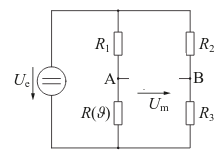
\includegraphics[scale=2.5]{katalog-1/a2-1.png}
  \end{center}
  Da die beiden Widerstandsäste parallel gescchaltet sind, muss über beiden Ästen die gleiche Spannung abfallen:
  \begin{center}
    $U_e = U_{R_1} + U_{R_\vartheta} = U_{R_2} +U_{R_3}$
  \end{center}
  Somit können wir die Spannung über $R_\vartheta$ mithilfe des Spannungsteilers berechnen:
  \begin{center}
      $U_{R_\vartheta} = U_e \cdot \frac{R_\vartheta}{R_1 + R_\vartheta}$
  \end{center}
  Die Leistung über einem Widerstand ist definiert als:
  \begin{center}
    $P_R = U_R \cdot I_R = \frac{U_R^2}{R}$
  \end{center}
  Somit gilt für die Leistung über dem Widerstand $R_\vartheta$ ;
  \begin{center}
      $P_{R_\vartheta} = \frac{U_{R_\vartheta}^2}{R_\vartheta} = (U_e \cdot \frac{R_\vartheta}{R_1 + R_\vartheta})^2 \cdot \frac{1}{R_\vartheta} =  \frac{U_e^2 \cdot R_\vartheta}{(R_1 + R_\vartheta)^2} $
  \end{center}

  Um den Maximalwert dieser Leistung in Abhängigkeit des Widerstandes $R_\vartheta$ herauszufinden, leiten wir die Leistung nach $R_\vartheta$ ab und setzen sie zu 0:
  \begin{center}
    $\frac{d}{dR_\vartheta}(P_{R_\vartheta}) \stackrel{!}{=} 0 \rightarrow R_\vartheta = R_1 = 1k \Omega$
  \end{center}
  Die benötigte Temperatur berechnet sich zu:
  \begin{center}
    $R(\vartheta) = 1k\Omega (1 + \alpha (\vartheta - \vartheta_0)) \stackrel{!}{=} 1k \Omega$ \\
    $\Rightarrow \vartheta = \vartheta_0 = 20$\textdegree
  \end{center}
  Für die Spannung $U_e$ erhalten wir:
  \begin{center}
    $50mW \stackrel{!}{=} P_{R_\vartheta} = U_e^2 \cdot \frac{1k\Omega}{4k\Omega}$ \\
    $\rightarrow 200mW = U_e^2$ \\
    $ \rightarrow U_e = 14.14V$
  \end{center}
  \item b) Für die Spannung $U_m$ können wir folgende Masche aufstellen:
  \begin{center}
    $U_m = U_{R_\vartheta} - U_{R_3}$
  \end{center}
  Wobei wir $ U_{R_\vartheta}$ und $U_{R_3} $ mit dem Spannungsteiler berechnen können:
  \begin{center}
    $U_{R_\vartheta} = U_e \frac{R_\vartheta}{R_\vartheta + R_1} $ \\
      $U_{R_3} = U_e \frac{R_3}{R_2 + R_3} $
  \end{center}
  Somit gilt für $U_m$:
  \begin{center}
    $U_m = U_e \big(\frac{R_\vartheta}{R_\vartheta + R_1}  - \frac{R_3}{R_2 + R_3} \big)$
  \end{center}
  Mit der Bedingung, $U_m(\vartheta = \vartheta_0 = 0 $\textdegree$) = 0V$ erhalten wir:

  \begin{center}
      $0V= U_e \big(\frac{R(\vartheta_0 )}{R(\vartheta_0) + R_1}  - \frac{R_3}{R_2 + R_3} \big) = U_e \big(\frac{0.9 k\Omega}{1.9 k\Omega}  - \frac{R_3}{R_2 + R_3} \big)$ \\
      $\rightarrow \frac{R_3}{R_2 + R_3} = \frac{0.9 k\Omega}{1.9 k\Omega}  $ \\
      $\rightarrow R_3 = \frac{0.9}{1.9} \cdot (R_2 + R_3) $
  \end{center}

  Für die Leistung gilt:
  \begin{center}
    $P_{(R_2,R_3)} = \frac{U_e^2}{R_2 + R_3}  \stackrel{!}{=} 10mW$ \\
    $\rightarrow (R_2 + R_3) = \frac{U_e^2}{10mW} = 14400\Omega$
  \end{center}
  Somit gilt:
  \begin{center}
    $R_3 = \frac{0.9 k\Omega}{1.9 k\Omega} \cdot (14400\Omega) = 6821.05 \Omega $ \\
    $R_2 = 14400\Omega - R_3 = 7578.95 \Omega$
  \end{center}


  \item c) Wir bezeichnen mit $U_{ideal}$ die Spannung bei idealer Messung und mit $U_{err}$ die Spannung mit ungenauen Widerständen.
  \begin{center}
    $U_{ideal} = 12V \big( \frac{R_\vartheta}{R_\vartheta + R_1} - \frac{R_3}{R_3 + R_2}\big)$ \\
    $U_{err} = 12V \big( \frac{R_\vartheta}{R_\vartheta + R_1' } - \frac{R_3'}{R_3'+R_2'}\big)$
  \end{center}
  Die Differenz ist:
  \begin{center}
    $F(R_\vartheta)) = U_{ideal} - U_{err} = U_e \big (\frac{R_\vartheta}{R_\vartheta + R_1 } -\frac{R_\vartheta}{R_\vartheta + R_1'} - \frac{R_3}{R_3 + R_2} + \frac{R_3'}{R_3'+R_2'})$
  \end{center}
  Der Fehler wird maximal, wenn die Differenz stark negativ wird. Dies ist der Fall, falls $\frac{R_3'}{R_3'+R_2'} < \frac{R_3}{R_3+R_2}$ und $  \frac{R_\vartheta}{R_\vartheta + R_1'} > \frac{R_\vartheta}{R_\vartheta + R_1}$  gilt. Somt gilt für die Widerstände:

   \begin{center}
     $R_3' < R_3 \rightarrow R_3' = 0.9 \cdot R_3$ \\
      $R_2' > R_2 \rightarrow R_2' = 1.1 \cdot R_2$ \\
      $R_1' < R_1 \rightarrow R_1' = 0.9 \cdot R_1$
   \end{center}
  Um die Temperatur herauszufinden, leiten wir die Differenz nach $R_\vartheta$ ab:
  \begin{center}
    $\frac{d}{d R_\vartheta} (F(R_\vartheta)) \stackrel{TR}{=} U_e \cdot \big( \frac{R_1}{(R_1 + R_\vartheta)^2} - \frac{R_1'}{(R_1' + R_\vartheta)^2}\big)\stackrel{!}{=} 0$ \\
    $\stackrel{TR}{\rightarrow} R_\vartheta = \sqrt{R_1 \cdot R_1'} = 0.949 \cdot R_1 = 949 \Omega$ \\
    $\rightarrow (1 + \alpha (\vartheta - \vartheta_0)) = 0.949  $ \\
    $\rightarrow \vartheta = 9.8$\textdegree
  \end{center}
  Der Betrag des Fehler berechnet sich zu:
  \begin{center}
      $ U_{err} = 12V \big( \frac{R_\vartheta}{R_\vartheta + R_1'} - \frac{R_3'}{R_3' + R_2'} \big) = 1.07V$ \\
      $ U_{ideal} \stackrel{!}{=} 1.07V \rightarrow R_\vartheta = $
  \end{center}
\end{itemize}
\end{homeworkProblem}




%----------------------------------------------------------------------------------------

\end{document}
